%%%%%%%%%%%%%%%%%%%%%%%%%%%%%%%%%%%%%%%%%%%%%%%%%%%%%%%%%%%%%%%%%%%%%%%%%%%%%%%%%%%%%%%%%%%
%                               Evaluation - 16pp
%%%%%%%%%%%%%%%%%%%%%%%%%%%%%%%%%%%%%%%%%%%%%%%%%%%%%%%%%%%%%%%%%%%%%%%%%%%%%%%%%%%%%%%%%%%
\chapter{Evaluation}
\label{sec:evaluation}

\section*{Summary}

In this chapter we will present and discuss the experimental evaluation made to Floodgate, along with its results. In first place, we will explain the evaluation methodology, and the reasons for its choice. Next, we will specifically present the test plans performed and the verified results, in the form of graphs, with mean and standard deviation values. Finally, we will discuss these results, presenting possible future optimizations.

The next chapter marks the end of this thesis, by presenting the conclusions regarding the developed work, along with some directions in terms of future work.

\section{Methodology}

Since Floodgate operates in an end-to-end fashion, in order to enforce data protection both on mobile and \textit{backend} sides, its evaluation must also be performed on both sides. To achieve that, we firstly performed quantitative isolation tests regarding the mobile and server sides, separately, with the goal of testing the overhead introduced by Floodgate on their performance. After that, and since the Floodgate's operation rely on network requests being made between the mobile and server sides, we performed quantitative integration tests where we evaluated the latency imposed by the system on these requests. Apart from that, we performed some tests in order to evaluate specific components of \textit{backend}-supported applications, like the server throughput and the performance of database operations. On the qualitative side, we performed two different tests. A fully-functional use-case application which shows all of Floodgate's features working together, and also a security evaluation of our system. Security regarding data storage and propagation over the network is a must-have in today's applications. All of our experiments were performed on the following hardware: For the mobile side, an LG Nexus 5 (2014), 2GB RAM, 16 GB storage. For the backend, a single-core 2GHz virtual machine running on an Hewlett-Packard BladeCenter, 2GB RAM, running Debian 7 64-bit and a Ceph-distributed storage of 5GB. Also, we used Oracle's ``HotSpot'' JVM \footnote{On Sect. \ref{sec:server-performance}, for the \textit{tradesoap} and \textit{tradebeans} benchmarks we used OpenJDK ``IcedTea'' JVM, version 1.7.0-79, due to some required classes not being present on Oracle's JVM.}, version 1.7.0-79 to support our server applications.

In summary,  we split our evaluation methodology in the following components:

\begin{itemize}
\item Quantitative evaluation
\begin{itemize}
\item Isolated performance impact
\begin{itemize}
\item Mobile-side performance impact
\item Server-side performance impact
\end{itemize}
\item Requests' latency decomposed on their factors (mobile-side, server-side and network)
\item Server throughput
\item Database operations (read/write) performance
\end{itemize}
\item Qualitative evaluation
\begin{itemize}
\item Use-case application
\item Security evaluation
\end{itemize}
\end{itemize}

\section{Mobile-side Performance Impact}
\label{sec:mobile-performance}

In this section we present the test plan and results of Floodgate's impact on the performance of mobile-side operation, along with a discussion regarding these results.

Floodgate's operation on the mobile-side consists in controlling the access and propagation of sensitive information concerning the user and the device itself. Due to that, to evaluate the mobile-side performance impact introduced by Floodgate, we compared the performance of accessing multiple sensitive information sources when in the presence and absence of Floodgate. Since Floodgate intercepts the access to these information sources and taints the application accordingly, verifying this taint on the subsequent network accesses, a substantial overhead was expected.

Our test plan consisted in accessing 10 different sensitive resources available through the Android APIs, and subsequently sending them through HTTP requests to the \textit{backend}. Each resource was previously set to "private" in the permissions manifest, and each access was performed in independent experiments, in order to guarantee no influence between accesses and minimal system load. Although, our experiments ended right before the requests are actually sent to the network, since this test only intends to measure the impact on the mobile-side operation. The 10 resources tested were: the device's GPS location, bluetooth address, IMEI, the SIM card phone number, serial number, IMSI, the network SSID and the user's country, timezone and saved accounts. We measured the time between calling the desired resource until getting the HTTP request ready to be sent. This way, we measure the performance of the whole Floodgate mobile-side operation. 

Figure \ref{fig:mobile-performance} presents the test results, by comparing the time to perform the operations described above.

The results show a high similarity between the experiments durations, except for the GPS location resource, since it requires an additional overhead caused by the Android framework asking for the location sensor refresh in order to get an updated device position. Also, the results show that Floodgate adds an average of 32\% overhead. This increase is due to a) the interception of the resource call, in order to verify the resource's privacy settings and subsequent application taint according to that; and b) interception of the network requests and the privacy header addition according to the application taint. We consider these results as acceptable, not harming the user experience with applications. Also, these results show that Floodgate imposes roughly the same mobile-side overhead as TaintDroid does, without modifying the underlying mobile operating system.

\begin{figure}[t!]
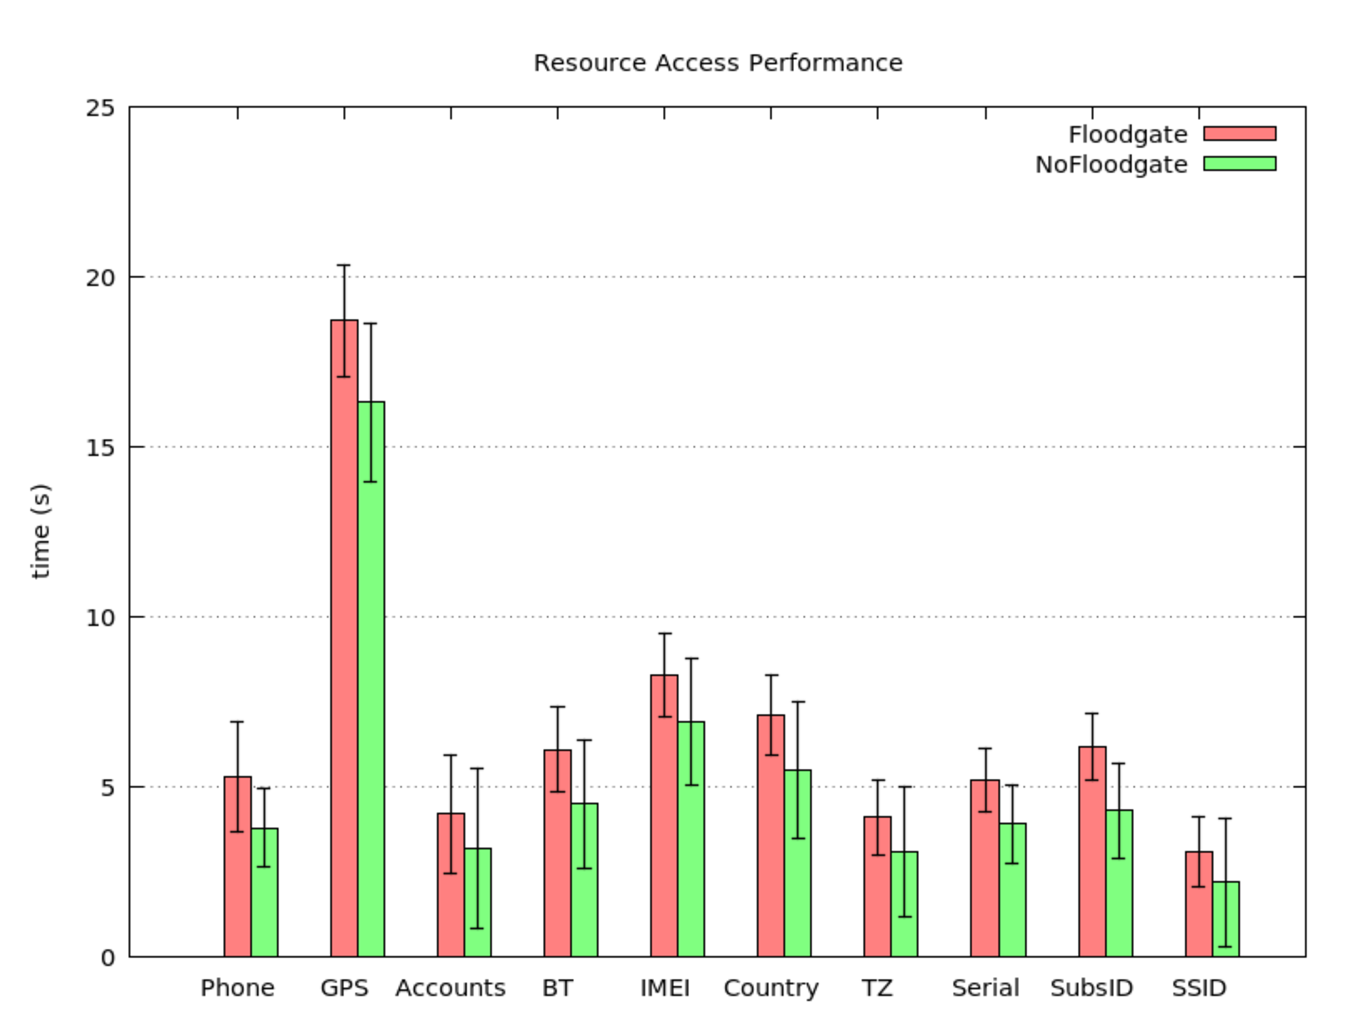
\includegraphics[width=\textwidth]{figs/mobile-performance}
\centering
\caption{Mobile-side performance impact}
\label{fig:mobile-performance}
\end{figure}

\section{Server-side Performance Impact}
\label{sec:server-performance}

Here we will present the test plan, results and respective discussion for evaluating Floodgate's impact on our backend.

To evaluate the impact of dealing with instrumented data and performing operations with this data on the server-side, we defined a metric to measure that impact: We chose the execution time and memory usage of server-side programs when in the presence of Floodgate. We focused our test plan on the DaCapo \footnote{\url{http://www.dacapobench.org/}} 9.12-bach macro-benchmark suite, which contains 14 benchmarks and simulates real-world applications within its workloads, manipulating multiple data types. All these benchmarks were ran using the \textit{``default''} size workload. We measured the execution time and maximum JVM heap usage. Due to the augmented number of instructions on the Floodgate-instrumented version of the programs, a substantial overhead was expected.
The test results are represented on Fig. \ref{fig:server-performance} and \ref{fig:server-memory}, for execution times and JVM heap usage, respectively.

\begin{figure}[t!]
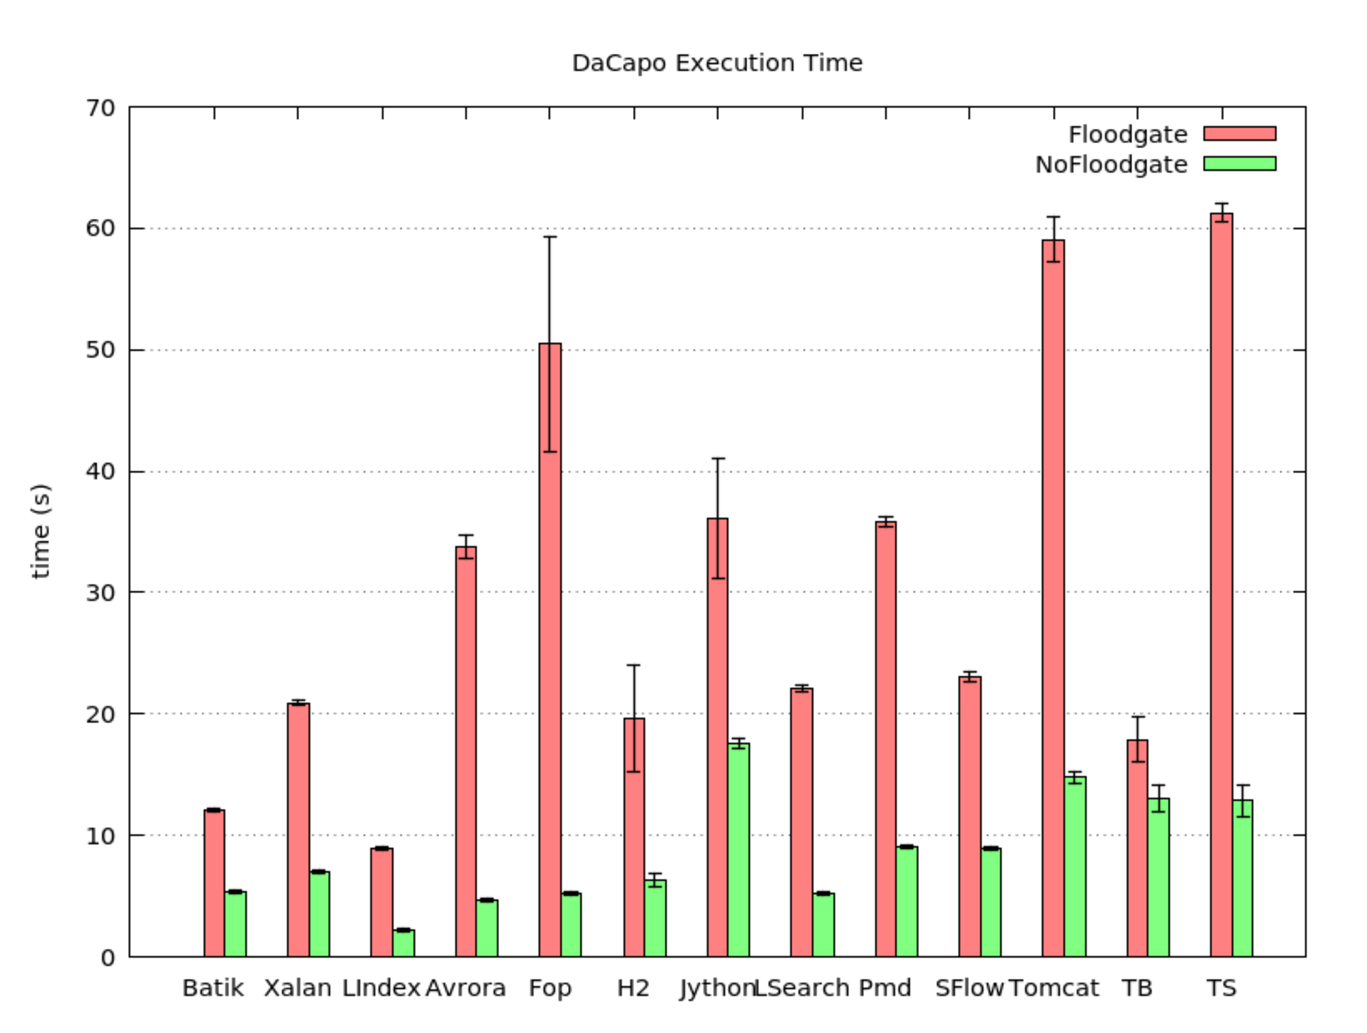
\includegraphics[width=\textwidth]{figs/server-performance}
\centering
\caption{Server-side performance impact}
\label{fig:server-performance}
\end{figure}

Analyzing the results, we spot that Floodgate introduces an overhead of about three times on the \textit{backend} performance. Despite it is a considerable value, each of the performed tests was specifically engineered to test different and heavy operations. Looking closely to Fig. \ref{fig:server-performance}, we can conclude that Floodgate behaves better in some of the tests than in others. Concretely, Floodgate introduced lower overhead values when executing the Batik or Xalan benchmarks. On the one side, the Batik benchmark consists in converting image files from \texttt{.png} to \texttt{.svg} format. The Xalan benchmark, on the other side, transforms XML into HTML documents. In opposition, the Fop or Avrora benchmarks introduced higher overhead values. Their execution consist in parsing an XSL-FO file and converting it to PDF, and simulating a number of programs running on a grid of AVR microcontrollers, respectively. In conclusion, Floodgate's \textit{backend} performance can prove itself better, depending on the kind of operations performed by the application at the server-side.

\begin{figure}[t!]
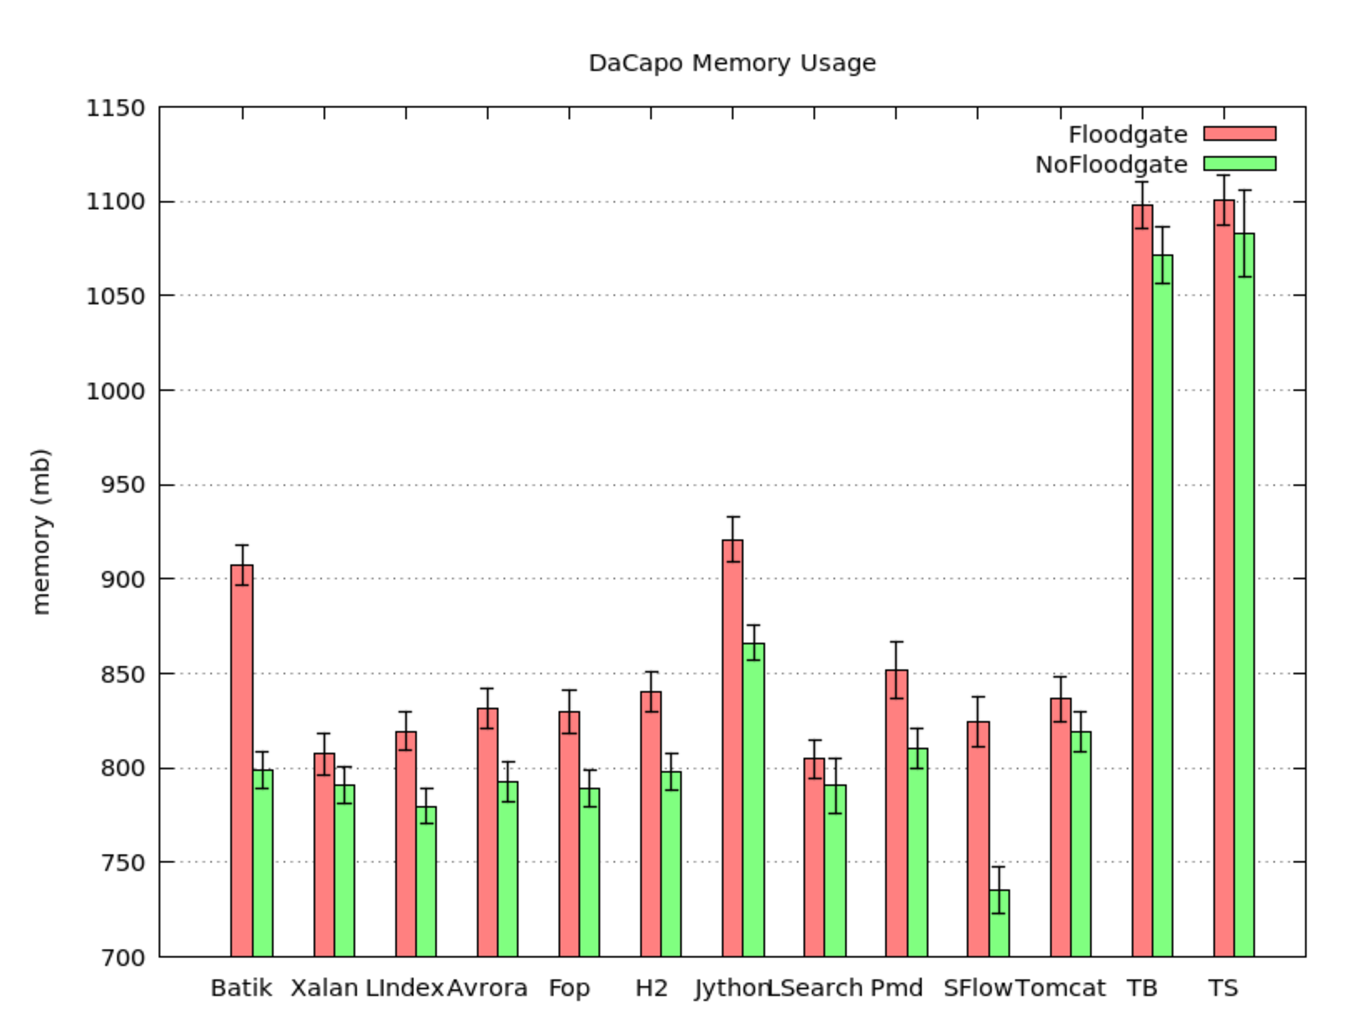
\includegraphics[width=\textwidth]{figs/server-memory}
\centering
\caption{Server-side memory usage impact}
\label{fig:server-memory}
\end{figure}

In contrast, the maximum memory heap usage test showed that Floodgate introduced an overhead of about 5.2\%, which we consider a great result. Since the performed tests were very resource-consuming, Floodgate server showed here some memory-usage efficiency.

\section{Mobile-server Interactions' Latency}
\label{sec:mobile-server-latency-eval}

Since Floodgate's target are \textit{backend}-supported mobile applications, which functionality rely on network requests made between mobile and server \textit{endpoints}, these requests' latency is also an important test metric to evaluate our system. These target mobile applications' functionality is often based on mobile \textit{endpoints} consuming resources (i.e. API methods) offered by a \textit{backend}. 

In this section, we will present a test plan, the respective results and critics, regarding the network requests' latency imposed by Floodgate during its operation.

So, to evaluate the request's latency imposed by Floodgate, we developed a simple application which works as a \textit{baseline} for test purposes. In the mobile endpoint, the application accesses the device's phone number and sends it through an HTTP request to the \textit{backend}. The \textit{backend}, by its turn, simply returns the same phone number, concatenated with the string ``ok!''. Finally, the mobile device prints the \texttt{<phone\_number> + ok!} message on the screen. 

Our test plan consisted in measuring the time spent by the three components we can spot here: The mobile endpoint, in which Floodgate controls the access to the phone number and generates the network request. The \textit{backend}, responsible for receiving the resource and generating the response. And the network, responsible for delivering the network request and returning the correspondent response. By comparing the Floodgate and the non-Floodgate versions, we expected increases in both the mobile-side and server-side components, due to Floodgate's operation, but similar measures in the network component. This is because all that Floodgate adds to the network requests is a ``privacy'' header, which we think is not a relevant addition in terms of time to deliver the requests.

The results for all the components' execution times are represented in Fig. \ref{fig:mobile-server-latency}.

\begin{figure}[t!]
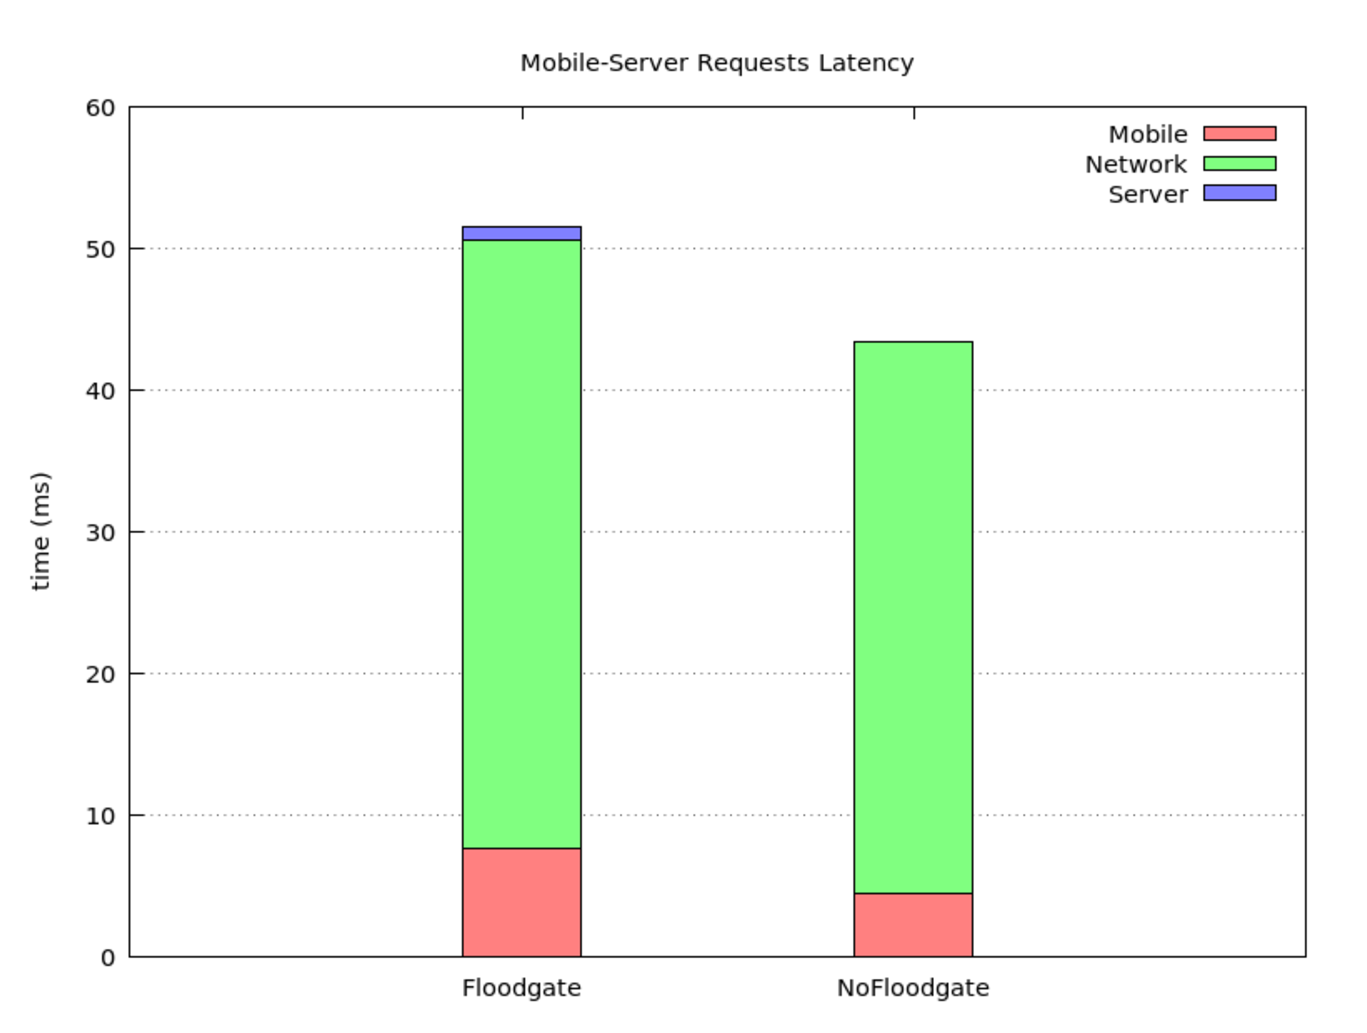
\includegraphics[width=\textwidth]{figs/mobile-server-latency}
\centering
\caption{Mobile-server latency}
\label{fig:mobile-server-latency}
\end{figure}

The results showed that Floodgate introduced an impact of about 69\% on the mobile-side performance, 10\% on the network component and also an overhead of about 400 times on the server-side performance.

On the mobile-side, the observed results somehow matched with the expected ones. In this test, we accessed the device's phone number and sent it through the network, measuring the execution time on the mobile-side only, just as we did on Sect. \ref{sec:mobile-performance} with multiple mobile resources. On that test, accessing the mobile phone number with Floodgate showed an overhead of about 40\%. Although, the test ended when the phone number privacy was added to the HTTP request's headers. In this test, the increased overhead may be justified in part by the time spent for the mobile device to process the HTTP response and present it on the mobile device's screen.

The network component, with an average overhead of 10\%, also makes us assuming it as a good result. Despite most Floodgate operation occurs both on the mobile and server-sides, we can justify the network overhead with the fact that, with Floodgate, each HTTP request will carry an additional HTTP header, the ``privacy''. Still, we consider that this result doesn't harm the practical user experience with Floodgate applications.

Finally, the server-side verified an excessive overhead of about 400 times. On Sect. \ref{sec:server-performance}, we already measured the server-side performance under heavy operations, which showed an overhead of about 300 times. Although, this time our \textit{backend} only executed a simple baseline operation of returning the input sent by the mobile device. Due to that, the execution times revealed themselves really small. The no-Floodgate version of the server spent an average of 0.0022 milliseconds to complete this task. Applying the Floodgate server instrumentation, this time increased to an average of 0.90 milliseconds. This way, we justify the giant overhead with the fact that it can easily occur when execution times are of these order of magnitude.

In conclusion, we consider these results as average ones, given that, in practice, we consider this doesn't prejudice the user experience with the application.

\section{Database Read/Write Operations Performance}

Another meaningful test plan we performed considered the performance of read/write operations of the \textit{backend} database, since all common application \textit{backends} have to persistently store their data. In this section, we will present the test plan and respective results that we prepared to test Floodgate applications' database performance. Floodgate, or concretely the Dropwizard framework, provides managed access to JDBI, a flexible and modular library for interacting with relational databases via SQL.

In this test plan, we took the simple application we created for the evaluation on \ref{sec:mobile-server-latency-eval} and created a simple database on our \textit{backend} that could handle the phone numbers arriving there. Also, we implemented a method on the mobile \textit{endpoint} application to query the database for the existing phone numbers. Here we measured the average time spent by Floodgate on two essential database operations: Writing a new phone number to the database; and reading the existing phone numbers, by querying the database.

\begin{figure}[t!]
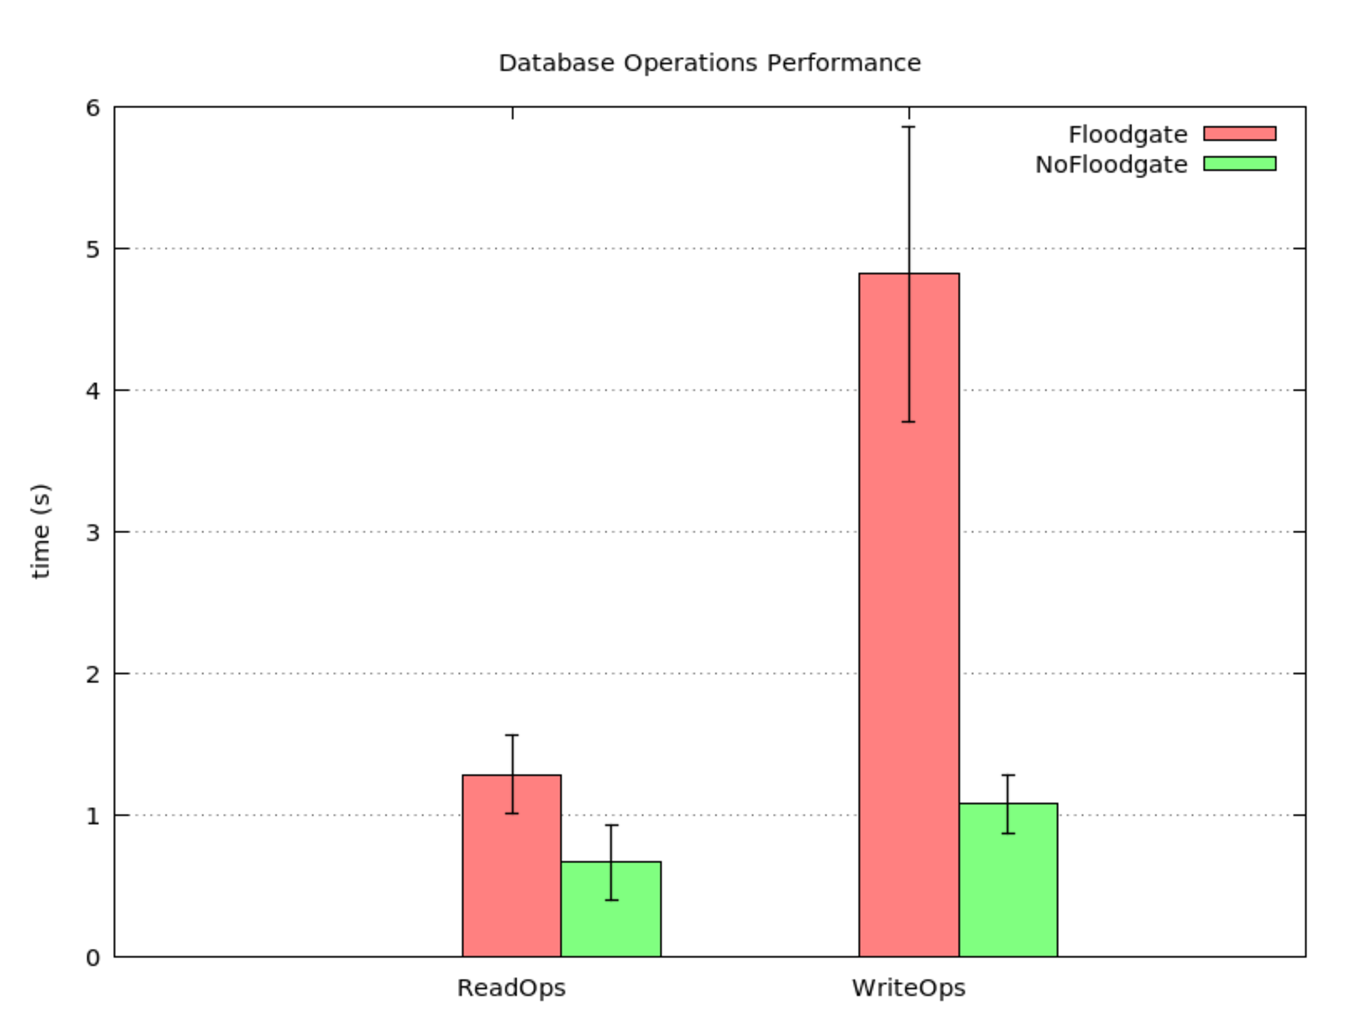
\includegraphics[width=\textwidth]{figs/database-performance}
\centering
\caption{Floodgate database performance}
\label{fig:database-performance}
\end{figure}

The results on Fig. \ref{fig:database-performance} show that Floodgate imposes an overhead of about 5.8 times when writing an object to the database, and an overhead of about 1.9 times when reading from the database.

During read operations, the verified results can be classified as extremely positive. This is because every time an object is read from the database on a Floodgate server, another query is automatically executed to our persistence taint module, in order to find the respective taint tag, and assign it to the object. This way, an overhead of 1.9 times matches the expected result. 

On the other side, write operations reveal a higher overhead (5.8 times). Just like in read operations, when an object is written to the database Floodgate provides, another object containing the first's taint tag must be written to the persistence taint database. So, we can conclude that Floodgate behaves worse during write operations, but the verified results somehow match the expected ones, since write operations to all common databases are more time-consuming, when compared to read operations.

\section{Use-case Application}

Apart from the quantitative evaluation we presented on above, Floodgate was also qualitatively evaluated. To do that, we developed an use-case application, with both mobile and \textit{backend} components, as near as possible to a real-world application which could at the same time provide a useful service to its users and show all the Floodgate's functionality. This way, we implemented AuctionsApp. As the name implies, it consists in an auctions app that allows users to post items for auctioning and live bidding on any available item except the ones they posted itself. 

To test Floodgate's operation, we developed a permissions manifest in which we declared the device's phone number as a private resource, and then we implemented an willful security flaw. For instance, every time a user puts a bid on any item, the mobile application will access the device's phone number, and send it through the network to the \textit{backend}, along with the bid's information. Here, Floodgate ensures that all the requests exchanged between the mobile and server sides will include the ``privacy'' header to state whether the request's content is tainted or not. 

On the server-side, the application receives the request and creates the bid, persistently storing the incoming information and updating the price of the item to which the bid applies. Also, Floodgate  filters the request, enforcing incoming taints to be applied to data, right before this data enters the \textit{backend's} application flow and enforces taints to be persistently stored at the same time as their correspondent data.

Every time a user asks for the list of current available items (whose auction periods haven't expired yet), it triggers an action on the Floodgate's server which can be decomposed on multiple parts: First of all, the application queries the persistent database for all the open auctions available. After that, Floodgate checks whether each one of these items have a correspondent persistent taints. If so, those taints are applied before the items leave the database and enter the application flow. After that, the application produces an HTTP response with the information of all available items and calls network methods to dispatch it. Although, this response will be filtered by the outcoming HTTP filters present on the \textit{backend}, in order to check whether the content being exported is, therefore, tainted. If it is, Floodgate is able to block the response or to let it proceed based on certain checks, to be defined by the programmer itself (i.e. destination endpoint, taint type, etc.).

\section{Security Evaluation}



    
 
